% #############################################################################
% This is Chapter 1
% !TEX root = main.tex
% #############################################################################
% Change the Name of the Chapter i the following line
\fancychapter{Introduction}
\clearpage
% The following line allows to ref this chapter
\label{chap:chap001}
\noindent

This section presents the work motivation, goals, and contributions of this dissertation thesis in the context of my doctoral program.
The work described in this document started in September 2015, before and during my Master Thesis, founded by a research grant from \ac{FCT}.
The funding was provided under the \ac{RD} Units Strategic Plan - 2013/2015 - \ac{OE}, with the UID/EEA/50009/2013 reference.
The official starting date of my \ac{PhD} program in \ac{CSE} at \ac{IST} of \ac{UL} is September 2018, and since January 2020, my work has been funded by \ac{FCT} with the grant PD/BD/150629/2020 reference.

\section{Motivation}
\label{sec:chap001001}

\textcolor{revised}{Breast cancer is ranked as the second leading cause of cancer-related deaths in women~\cite{doi:10.1002/cncr.32859}, and calls for effective screening and diagnostic methods~\cite{https://doi.org/10.3322/caac.21754}.
Screening is typically recommended for women aged 40 to 50~\cite{https://doi.org/10.3322/caac.21754}.
The need for improved diagnostic methods is underscored by over 400,000 new European cases annually and the variability in diagnostic accuracy among clinicians~\cite{Dafni2019}, further complicated by the complexities of image interpretation (Figure~\ref{fig:fig114}).
This dissertation focuses on integrating \ac{AI} into medical imaging to refine diagnostic procedures and reduce inaccuracies.}

%%%%%%%%%%%%%%%%%%%%%%%%%%%%%%%%%%%%%%%%%%%%%%%%%%%
\begin{figure}[ht]
\centering
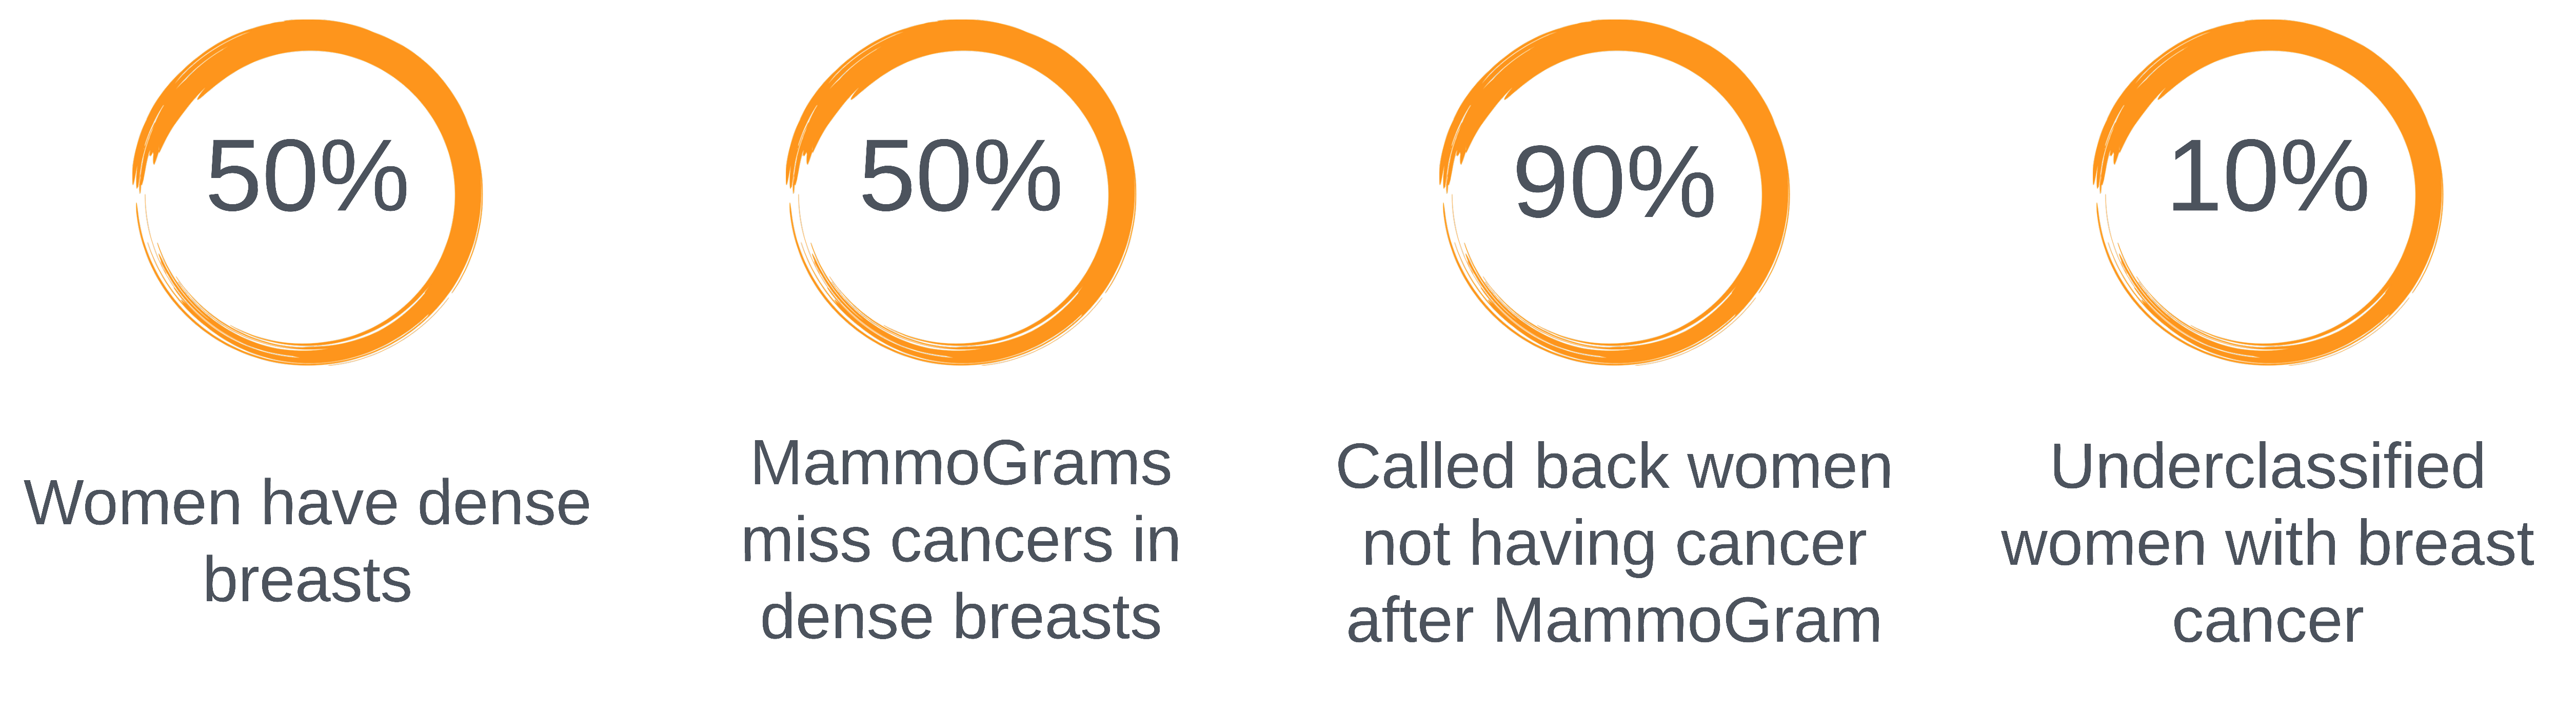
\includegraphics[width=\textwidth]{images/fig114}
\caption{\textcolor{revised}{Breast cancer patient proportions with missed cases vary in screenings. About half of women have dense breasts, which can obscure 50\% of cancers. FPs are common in breast screenings; approximately 90\% of women recalled for further exams after a mammogram don't have cancer. Moreover, around 10\% of breast cancers are wrongly classified as negative (FN) but are positive, posing serious risks for patients. Source: National Cancer Institute (\href{https://www.cancer.gov/types/breast/mammograms-fact-sheet}{cancer.gov}). Retrieved on July 3, 2023.}}
\label{fig:fig114}
\end{figure}
%%%%%%%%%%%%%%%%%%%%%%%%%%%%%%%%%%%%%%%%%%%%%%%%%%%

\textcolor{revised}{A pivotal aspect of this integration is medical professionals' acceptance of \ac{AI} systems.
Guided by the \ac{UTAUT}\cite{CALISTO2022102922, info:doi/10.2196/27122} model, this research investigates factors influencing clinicians' willingness to embrace \ac{AI} in their workflows, a fundamental step in realizing \ac{AI}'s potential in healthcare\cite{10.1001/jamainternmed.2015.5231, Houssami2017}.
It examines the utility and impact of \ac{AI} on clinical decision-making~\cite{9473208}.
The study also assesses how security, risk, and trust impact \ac{AI} adoption in healthcare, especially within \acp{CDSSe} integrated into the \ac{RRR}, aligning with clinicians' needs to improve patient care~\cite{10.1145/3544548.3581075, EVANS2022281}.}

\textcolor{revised}{Recent research advocates a shift in \ac{AI} towards collaboration, surpassing human diagnostic capabilities~\cite{Ribli2018, Topol2019}.
Technologies like {\it radiomics}, \ac{CADe}, and \ac{CADx} are crucial amid the medical professional shortage~\cite{McKinney2020}.
This work is using a human-centered approach~\cite{doi:10.1148/radiol.2019182627}, customizing \ac{AI} to clinicians' needs and addressing transparency, countering the traditional opacity issue~\cite{10.1145/3306618.3314293}.
In this paradigm, \ac{HAII} enhances the interaction between humans and \ac{AI} systems, leveraging their strengths for effective decision-making~\cite{10.1145/3313831.3376807, 10.1145/3313831.3376301}.}

\textcolor{revised}{In addressing the `black box' nature of \ac{AI} in \ac{DL}~\cite{10.1145/3306618.3314293}, such as the \acp{CNN} used under this thesis~\cite{10230448, 10230686}, the focus is on transparent decision-making and enhancing clinician-\ac{AI} collaboration.
Mimicking clinicians' reasoning by aligning \ac{AI} recommendations with their expertise levels ensures consistency with their decision processes~\cite{Tschandl2020}.
The dissertation highlights assertiveness-based communication in \ac{AI} systems for collaboration~\cite{pacheco2019alignment, 10.1145/3544548.3580682}.
This approach improves diagnostic accuracy and reduces \acp{FP}\cite{10.1001/jamainternmed.2014.981} and \acp{FN}\cite{doi:10.1056/NEJMe1912943}, bridging the gap between \ac{AI}'s capabilities and healthcare professionals' needs.}

\textcolor{revised}{This dissertation is centered on the design and integration of \ac{AI} systems to enhance medical imaging for breast cancer detection.
It aims to significantly boost diagnostic accuracy, decrease \ac{FP}\footnotemark[1] and \ac{FN}\footnotemark[2] rates, as well as improve overall healthcare efficiency.
Utilizing anthropomorphic intelligent agents with personalized \ac{AI} communication, the research intends to advance clinical diagnostics.
This effort, merging innovative technology with professional expertise, is geared towards increasing diagnostic precision, optimizing healthcare operations, reducing errors, and ultimately achieving better outcomes for patients.}

%%%%%%%%%%%%%%%%%%%%%%%%%%%%%%%%%%%%%%%%%%%%%%%%%%%
\footnotetext[1]{\textcolor{revised}{False-Positive: when the screening result appears abnormal, requiring further tests to confirm cancer. FP results are more common in younger women with dense breasts, previous breast biopsies, a family history of breast cancer, or estrogen use.}}
%%%%%%%%%%%%%%%%%%%%%%%%%%%%%%%%%%%%%%%%%%%%%%%%%%%

%%%%%%%%%%%%%%%%%%%%%%%%%%%%%%%%%%%%%%%%%%%%%%%%%%%
\footnotetext[2]{\textcolor{revised}{False-Negative: when the screening result appears normal despite breast cancer being present, particularly in women with dense breasts. FN cases can falsely reassure women, implying they are cancer-free when, in reality, they have the disease.}}
%%%%%%%%%%%%%%%%%%%%%%%%%%%%%%%%%%%%%%%%%%%%%%%%%%%

\section{Thesis Statement}
\label{sec:chap001003}

\noindent
This dissertation aims to defend the following thesis statement:

\begin{quote}
{\it
\textcolor{revised}{Integrating anthropomorphic intelligent agents in \ac{AI}-powered medical imaging will significantly transform breast cancer detection outcomes.
Guided by the \ac{UTAUT} model, this dissertation initially examines the factors influencing system adoption among medical professionals, focusing on enhancing clinician workflows for improved diagnostic efficiency and accuracy.
It explores a user-centric approach to augment clinicians' diagnostic capabilities and emphasizes human-centered design in \ac{AI} system development to manage radiologists' workload and boost diagnostic confidence.
The study then investigates assertiveness-based strategies in adapting the communication of these agents for personalized medicine, tailoring \ac{AI} recommendations and explanations to align with radiologists' demographic characteristics, a fundamental factor in achieving effective, customized communication.
Anticipated outcomes include a fourfold increase in diagnostic speed, a 26\% reduction in medical errors, and a notable improvement in cancer detection rates, up to 95\% of accuracy, advancing healthcare efficiency.
The thesis posits that \ac{AI}'s successful adoption and integration in medical imaging depends on technological refinement and synergizing with user elements of medical practice.
It sets a new standard for \ac{AI} in healthcare and marks a shift towards more personalized and customized approaches.}
}
\end{quote}

\noindent
To defend this statement, the remainder of this dissertation addresses the following research questions:

\begin{enumerate}
\item How can intelligent agents be successfully designed, motivating clinicians to accept and adopt \ac{AI}-based systems in radiology?
\begin{enumerate}
\item How do the factors influencing clinicians' acceptance and adoption of intelligent agents in radiology manifest in practice?
\item How do clinicians perceive the potential benefits and drawbacks of adopting intelligent agents in radiology?
\item How can we design and implement effective strategies for encouraging clinicians' acceptance and adoption of intelligent agents in radiology?
\end{enumerate}
\item How can \ac{AI} assistance be designed and implemented to effectively improve the clinical workflow and diagnostic interpretability for clinicians in radiology?
\begin{enumerate}
\item How can we incorporate design interventions to effectively introduce \ac{AI} systems and enhance clinicians' satisfaction, acceptance, and overall experience with intelligent agents in radiology?
\item How should explainability be designed for setting appropriate expectations of clinicians and to improve diagnostic interpretability over an AI recommendation?
\item How does AI assistance impact clinicians' workflow for avoiding different types of diagnostics?
\end{enumerate}
\item How can personalization and customization be optimized to enhance medical assessments and improve clinicians' perceptions of the intelligent agents?
\begin{enumerate}
\item How does a personalized and customized intelligent agent affect medical assessments?
\item How do clinicians perceive a personalized and customized intelligent agent?
\end{enumerate}
\end{enumerate}

\section{Main Research Contributions}
\label{sec:chap001005}

\textcolor{revised}{This thesis explores the integration of intelligent agents in multimodal\footnotemark[3] medical imaging strategy, addressing user acceptance, design, and clinical applicability.
It evaluates a {\it BreastScreening} prototype in diverse clinical settings and offers design insights for {\it radiomics} in breast cancer.
The study also examines \ac{AI} communication strategies to improve clinical workflows and personalize \ac{AI} recommendations.
Additionally, it contributes comprehensive datasets for multidisciplinary research.
Appendix~\ref{chap:app001} provides more information about a further research view of the thesis (Section~\ref{sec:chap001002}), as well as the relationship between the problems and the contributions (Section~\ref{sec:chap001004004}) that the thesis is solving.}

%%%%%%%%%%%%%%%%%%%%%%%%%%%%%%%%%%%%%%%%%%%%%%%%%%%
\footnotetext[3]{Multimodality: in this thesis, a diagnostic technique for the patient: (1) \ac{MG}, both \ac{CC} and \ac{MLO} views; (2) \ac{US}; (3) \ac{MRI}; and (4) text. The considered text modalities are, for instance, report information, personal history, family history, and age, among others.}
%%%%%%%%%%%%%%%%%%%%%%%%%%%%%%%%%%%%%%%%%%%%%%%%%%%

\noindent
The main contributions achieved so far are the following:

\begin{enumerate}
\item {\bf Factors affecting the acceptance and adoption} of intelligent agents in medical imaging;
\begin{enumerate}[label*=\arabic*.]
\item Investigated {\bf factors affecting the adoption of intelligent agents in medical imaging}, verifying security, risk, and trust as essential antecedents of user acceptance;
\item Identified {\bf moderating relationships} between antecedent factors and behavioral acceptance based on gender, age, and education, between others, exploring how medical experience, training levels, and expertise areas can also moderate these relationships;
\end{enumerate}
\item {\bf Design and evaluation of intelligent agents} in real-world clinical settings;
\begin{enumerate}[label*=\arabic*.]
\item Conducted a study with 45 physicians, evaluating a {\bf BreastScreening prototype} with and without \ac{AI}, and compared the accuracy of the \ac{AI} condition using \ac{FP} and \ac{FN} metrics;
\item Provided {\bf design recommendations} for visualization to support {\it radiomics} in breast cancer;
\item Demonstrated the {\bf impact of multi-modal imaging and \ac{AI}-assisted strategy} in diagnosing and severity classification of lesions;
\item Examined the impact of our {\bf proposed design techniques} on clinicians' expectations and satisfaction when interacting with an intelligent agent;
\end{enumerate}
\item Enhancing clinical workflows and trust through {\bf assertiveness-based agents};
\begin{enumerate}[label*=\arabic*.]
\item Customized \ac{AI}-assisted medical reasoning with {\bf assertiveness-based communication}, enhancing clinical workflows;
\item Probes into the applicability of granular clinical explanations and user confidence in {\bf personalized \ac{AI} recommendations} without undermining diagnostic accuracy;
\item Explored the impact of explaining \ac{AI} outputs on medical efficiency, considering the {\bf communication tone} of clinical arguments;
\item Provided {\bf design considerations for adapting communication} in \ac{AI} reasoning based on medical expertise levels, facilitating the implementation of personalized intelligent agents;
\end{enumerate}
\item We {\bf published novel datasets} containing clinical information, user data, and results.
\end{enumerate}

\vspace{2.00mm}

\textcolor{revised}{In summary, this thesis significantly advances the integration of intelligent agents in multimodal medical imaging, focusing on user acceptance and trust.
Evaluating the designed prototypes in clinical settings, providing key insights and design recommendations for \ac{AI}-assisted diagnostics.
The introduction of assertiveness-based \ac{AI} communication enhances clinical workflows and personalizes care.
Additionally, the release of comprehensive datasets encourages further research.
This work underpins future advancements in medical imaging and \ac{AI}, demonstrating practical applications in healthcare.}

\section{\textcolor{revised}{Thesis Overview}}
\label{sec:chap001004}

This section outlines the main chapters of the thesis (Section~\ref{sec:chap001004001}), augmented with additional descriptions (Section~\ref{sec:chap001004002}) and supplementary materials (Section~\ref{sec:chap001004003}).
It concludes with a comprehensive summary of the section (Section~\ref{sec:chap001004005}).

\subsection{Thesis Core}
\label{sec:chap001004001}

Provided below is a comprehensive breakdown of the thesis, organized into its core chapters:

\vspace{2.00mm}

\noindent
{\bf Chapter~\ref{chap:chap002}}:
We provide a concise overview of the medical imaging background and the current clinical workflow.
We aim to highlight the opportunities for research and development of intelligent agents in this medical workflow.
Additionally, Appendix~\ref{chap:app001} extends a more comprehensive elaboration of the chapter.

\vspace{2.00mm}

\noindent
{\bf Chapter~\ref{chap:chap003}}:
This chapter of our dissertation offers a thorough literature review and explores recent developments in the field of \ac{HCI} about \ac{AI}-assisted medical decision-making.
In conjunction with Chapter~\ref{chap:chap002} and Appendix~\ref{chap:app001}, this chapter accomplishes our literature review goal.
Together, these components provide valuable insights into the medical background and critically analyze the relevant \ac{HCI} literature.

\vspace{2.00mm}

\noindent
{\bf Chapter~\ref{chap:chap004}}:
The chapter explores factors influencing clinicians' adoption of \ac{AI} in the medical workflow.
In conjunction, Appendix~\ref{chap:app002} expands a complete analysis to complement this chapter.
These components collectively address the acceptance and adoption challenges in medical imaging.

\vspace{2.00mm}

\noindent
{\bf Chapter~\ref{chap:chap005}}:
Explore radiologists' requirements in utilizing \ac{AI}-powered image diagnostics.
Appendix~\ref{chap:app003} offers additional insights to complement this chapter.
It is also essential to address Appendix~\ref{chap:app004}, which discusses the integration of our \ac{DL} models and their architectural implications for designing the final solution.
Jointly, these three components address the challenges related to our human-centered approach.

\vspace{2.00mm}

\noindent
{\bf Chapter~\ref{chap:chap006}}: This chapter explores how \ac{AI} systems should communicate to effectively address the specific needs and characteristics of different user groups.
In addition to this chapter, Appendix~\ref{chap:app005} provides supplementary insights.
Concurrently, these two components tackle the challenges associated with the personalization and customization of intelligent agents in clinical workflows.

\vspace{2.00mm}

\noindent
{\bf Chapter~\ref{chap:chap007}}:
Presents contributions and design recommendations under this thesis.
The findings emphasize the significance of compliant agents providing tailored explanations for future enhancements.
These insights contribute significantly to research in \ac{HCI} and \ac{AI} communication for healthcare.

\vspace{2.00mm}

\noindent
{\bf Chapter~\ref{chap:chap008}}:
Deliver the concluding findings of the dissertation, highlighting design principles.
Combined with Chapter~\ref{chap:chap007}, these chapters pave the way for \ac{AI} integration in healthcare.
Together, they address the final remarks and contributions of this dissertation.

In this section, we offered the core skeleton of the thesis.
We explored the relevant background context and pertinent literature that form the foundation for our work (Chapter~\ref{chap:chap002} and Chapter~\ref{chap:chap003}).
Subsequently, we presented chapters that contribute to our objective of enhancing the adoption of intelligent agents (Chapter~\ref{chap:chap004}) through a human-centered design approach (Chapter~\ref{chap:chap005}) and personalizing clinicians' decision-making (Chapter~\ref{chap:chap006}).
Finally, we discussed (Chapter~\ref{chap:chap007}) and concluded (Chapter~\ref{chap:chap008}) our main findings, revealing general design recommendations and principles.
For a more detailed discussion on how the thesis addresses specific problems and its contributions, refer to Section~\ref{sec:chap001004004} in Appendix~\ref{chap:app001}.

\subsection{Additional Descriptions}
\label{sec:chap001004002}

In this section, we briefly summarize the dissertation's core chapters, focusing on our main contributions for ease of understanding.
This concise overview clearly outlines our research journey, emphasizing key themes and findings.
Furthermore, it guides the in-depth explorations and comprehensive discussions detailed in the subsequent appendices, ensuring a coherent and structured progression of ideas throughout the dissertation.

\vspace{2.00mm}

\noindent
For more detailed insights, the following appendices are presented:

\vspace{2.00mm}

\noindent
{\bf Appendix~\ref{chap:app001}}:
This appendix extensively elaborates on topics from Chapter~\ref{chap:chap001} and Chapter~\ref{chap:chap002}, enriching understanding.
It offers practical insights for healthcare professionals seeking a deeper understanding of clinical processes.

\vspace{2.00mm}

\noindent
{\bf Appendix~\ref{chap:app002}}:
This appendix provides a comprehensive analysis and further findings on the acceptance and adoption of new technologies, extending the discussion from Chapter~\ref{chap:chap004}.
It delves into healthcare technology integration, shedding light on moderating factors, and is a valuable resource for policymakers and healthcare practitioners navigating \ac{AI} adoption.

\vspace{2.00mm}

\noindent
{\bf Appendix~\ref{chap:app003}}:
Delivers a detailed exploration of diagnostic performance and accuracy, furthering the discussions from Chapter~\ref{chap:chap005}.
This detailed exploration deepens insights into diagnostic performance and provides a roadmap for future research in medical imaging.
Readers gain a complete understanding of the practical implications of the research.

\vspace{2.00mm}

\noindent
{\bf Appendix~\ref{chap:app004}}:
Alongside Appendix~\ref{chap:app003}, this appendix provides valuable insights into the design process, specifically focusing on integrating \ac{DL} models.
This integration plays a pivotal role in the discussions in Chapter~\ref{chap:chap005}, forming a central component of the thesis exploration.
It offers crucial guidance for researchers and developers seeking to harness the potential of \ac{AI} for improved healthcare outcomes.

\vspace{2.00mm}

\noindent
{\bf Appendix~\ref{chap:app005}}:
This appendix expands upon the discussions in Chapter~\ref{chap:chap006} by providing additional results and in-depth discussions.
It includes valuable insights into clinicians' performance, preferences, and other pertinent aspects, informing future developments and research in healthcare \ac{AI}.

As this dissertation unfolds, each appendix plays a critical role in enriching and extending the discussions presented in the main chapters (Section~\ref{sec:chap001004001}).
The core chapters and appendices form a comprehensive and cohesive body of work (Section~\ref{sec:chap001004004} of Chapter~\ref{chap:app001}).
Not only do they store detailed information and analysis, but they also enhance the overall comprehension of our research findings.

\subsection{Complementary Information}
\label{sec:chap001004003}

In addition, we supplement the thesis with complementary information to provide readers with a more comprehensive understanding of our research.
This information will give further details concerning the used questionnaires, \ac{UTA} guides, and {\it framework} details, described next, ensuring a well-rounded exploration of our work and facilitating a deeper engagement with the dissertation's content.
These supplementary materials serve as valuable resources for researchers and practitioners seeking to delve into the intricacies of our study.

\vspace{2.00mm}

\noindent
To delve deeper into these specific topics, the subsequent appendices are provided:

\vspace{2.00mm}

\noindent
{\bf Appendix~\ref{chap:app006}}:
The employed questionnaires, {\it e.g.}, demographic data, \acs{SUS}, etc., are provided.
These questionnaires constitute a part of the outcomes derived from Chapter~\ref{chap:chap004}, Chapter~\ref{chap:chap005}, and Chapter~\ref{chap:chap006}.

\vspace{2.00mm}

\noindent
{\bf Appendix~\ref{chap:app007}}:
\ac{UTA} refers to a document that guides the user testing process.
The first document is connected to our 8\textsuperscript{th} \ac{UTA} for Chapter~\ref{chap:chap004}, the second to our 7\textsuperscript{th} \ac{UTA} for Chapter~\ref{chap:chap005}, and the third to our 11\textsuperscript{th} \ac{UTA} for Chapter~\ref{chap:chap006}.
The number progression follows the order of the chapters, not chronological.


\vspace{2.00mm}

\noindent
{\bf Appendix~\ref{chap:app008}}:
This complementary information attaches the technical report that sustains the invention of our basic {\it BreastScreening} framework~\cite{10.1145/3399715.3399744, WO2022071818A1}.
The document provides functionality details and market perspectives for introducing \ac{AI} systems in the healthcare sector.

\subsection{Summarizing Thesis Overview}
\label{sec:chap001004005}

In this section, we provide a comprehensive overview of our dissertation research. The central part of the dissertation comprises dedicated chapters (Section~\ref{sec:chap001004001}), each meticulously crafted to substantiate our thesis statement and contribute to our overarching research goals.
Furthermore, we offer more detailed insights into these chapters through additional descriptions (Section~\ref{sec:chap001004002}), focusing on elucidating the primary contributions, ensuring clarity, and guiding the reader through more detailed subjects and findings of our work.
Complementary information (Section~\ref{sec:chap001004003}) supplements the main research content, including questionnaires, \ac{UTA} guides, and technical details of the {\it framework}, along with its current market status, enhancing the reader's understanding of our work and its practical applications.
These supplementary materials are thoughtfully included alongside each chapter to address specific research challenges and provide comprehensive context for our findings and contributions (Section~\ref{sec:chap001004004}).